\section{Implementation}
\label{sec:implementation}

Current section covers technical details of the implementations of the tool. It covers module abstractions of the system, overview of the tools that were used during the development and
short discussions about the reasons as well.

\subsection{Programming Language and Tools}

Main language and platform for developing thesis is Java. Java is a programming language and computing
platform first released by Sun Microsystems in 1995. It is the underlying technology that powers state-of-the-art
programs including utilities, games, and business applications. Java runs on more than 850 million personal computers worldwide,
and on billions of devices worldwide, including mobile and TV devices.~\cite{java_com}
Also, there are a lot of different libraries in Java. Every common part of the system could be replaceable.
In the future sections would be detailed overview libraries for graphs, graph visualizations and graphic libraries.


Java is flexible platform which has big amount of different libraries. It helps not to write twice things already made but flexibility cause project structure complexity and library management. On the early stage there are no problems to control project throw sophisticated IDE (integrated development environment) but as project complexity grows more powerful building tool need appears. Maven is used during thesis work.


Maven~\cite{MAVEN_HOME_PAGE} is free, open-source and de-facto project management standard on the Java platform,
is part of Apache software project developed and supported by ASF (Apache Software Foundation)~\cite{APACHE_FOUNDATION_HOME_PAGE}.

\begin{quotation}
``Maven provides a comprehensive approach to managing software projects.
From compilation, to distribution, to documentation, to team collaboration,
Maven provides the necessary abstractions that encourage reuse and take much of the work out of project builds.''~\cite{MAVEN_BOOK_1}
\end{quotation}

Maven is a set of standards, a repository format, and a piece of software used to manage and describe projects.
It defines a standard life cycle for building, testing, and deploying project artifacts.
It provides a framework that enables easy reuse of common build logic for all projects following Maven's standards.
The Maven project at the Apache Software Foundation is an open source community which produces software tools that
understand a common declarative Project Object Model (POM).~\cite{MAVEN_BOOK_2}


Maven's primary goal is to allow a developer to comprehend the complete state of a development effort in the shortest period of time. In order to attain this goal there are several areas of concern that Maven attempts to deal with:
\begin{itemize}
	\item making the build process easy
	\item providing a uniform build system
	\item providing quality project information
	\item providing guidelines for best practices development
	\item allowing transparent migration to new features
\end{itemize}


In Figure~\ref{fig:THESIS_FOLDER_STRUCTURE} is the structure of the project folder. Thesis project uses standard Maven project folder format. Here is overview of key parts: java source code stored in the ``src/main/java'' folder, tests source code stored in the ``src/test/java''. Necessary resources such as log4j configuration file stored in the ``src/main/resources'', in the same folder thesis properties file is stored. During ``package'' phase all resources are copied by Maven.


``Native'' directory stores JOGL native libraries to different platform such as Linux, Windows and Mac OS X. In the ``lib.zip'' stored jars for JUNG library which should be manually placed in the local Maven repository because they do not  exist in central Maven repository. All other dependencies are exist in Maven repositories and handled by default dependency process.


Complete builds are stored in the ``build'' folder. Latest build stored in the ``build/latest'' folder, other builds stored in the folder that has such name pattern:


\texttt{GoClusterViz-\%version\%-\%build date\%-\%build time\%}


Each build folder contains corresponded native build for each of three platforms Linux, Windows and Mac OS X. Cluster graph and Gene Ontology graphs are stored in the ``data'' folder.

\begin{figure}[h!]
\centering
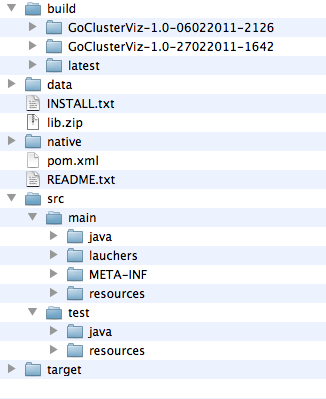
\includegraphics[scale=0.6]{pictures/thesis_folder_structure.png}
\caption{Thesis folder structure}
\label{fig:THESIS_FOLDER_STRUCTURE}
\end{figure}

Second necessary part of the normal development process is revision control.

\begin{quotation}
``Revision control, also known as version control or source control (and an aspect of software configuration management or SCM),
is the management of changes to documents, programs, and other information stored as computer files.
It is most commonly used in software development, where a team of people may change the same files.
Changes are usually identified by a number or letter code, termed the `revision number', `revision level', or simply `revision'.
For example, an initial set of files is `revision 1'. When the first change is made, the resulting set is `revision 2', and so on.
Each revision is associated with a time stamp and the person making the change. Revisions can be compared,
restored, and with some types of files, merged.''~\cite{REVISION_CONTROL}
\end{quotation}

During thesis development Git version control system was used.

\begin{quotation}
``Git is a distributed revision control system with an emphasis on speed.
Git was initially designed and developed by Linus Torvalds for Linux kernel development.
Every Git working directory is a full-fledged repository with complete history and full revision tracking capabilities,
not dependent on network access or a central server. Git is free software distributed under the terms of the
GNU General Public License Version 2.''~\cite{GIT}
\end{quotation}

Git allows to store and work locally on the machine but for safety reasons all source code stored on GitHub.
GitHub is a web-based hosting service for software development projects that use the Git revision control system.
GitHub provides free hosting for open-source project. Thesis project home page on GitHub~\cite{GitHub_homepage} and Git repository URL~\cite{GitHub_repository}.

\begin{figure}[h!]
\centering
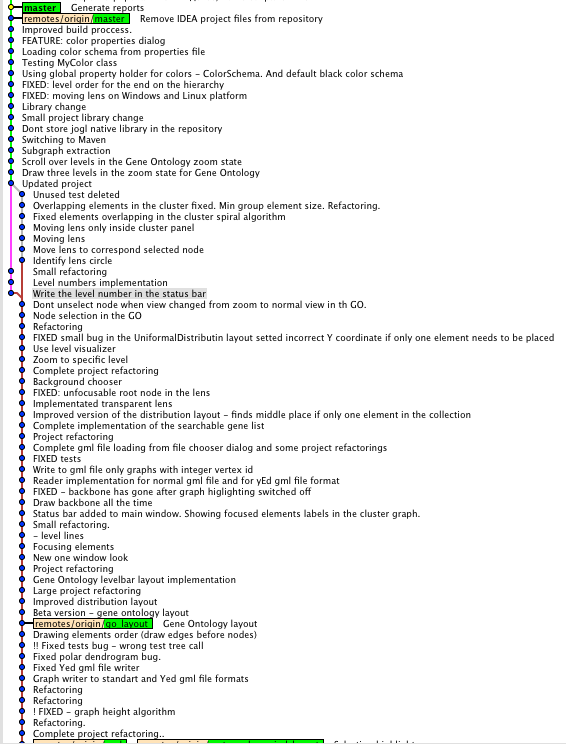
\includegraphics[scale=0.6]{pictures/commit_graph_gitk.png}
\caption{Commit graph of the local repository made by gitk tool}
\end{figure}


\subsection{Java Graph Libraries Overview}


There are overview of a few libraries for working with graphs in Java

\begin{enumerate}

\item
Java Graph Editing Framework (GEF)~\cite{GEF}

The aim of project consists in generation of library for graph editing, which can be used for construction of high-end (high-quality) custom applications for working with graphs.
GEF facilities (opportunities):
\begin{itemize}
	\item simple and clear design, which allows a developer to expand library's functionality
	\item Node-Port-Edge model of graph's presentation, which permits to perform overwhelming majority of tasks occurring in working with graphs applications
	\item future XML-based format support (SVG)
\end{itemize}

\item
ILOG JViews~\cite{ILOG_Jview}

ILOG JViews gives (grants) components, aimed for using in custom applications, and also in common with Ajax and Eclipse platform.

\item
JGraphT~\cite{JGraphT}

JGraphT is open source library, which provides with mathematical tool of graphs theory. JGraphT supports different kinds of graphs, including: oriented and unoriented graphs, graphs with weighted/non weighted/nominate (named) or anything else arc format, appointed 	by user, non upgradeable graphs - supported access to internal graphs in ``Read Only'' mode. Listenable graphs: allows outer listener to trace events appearance; sub-graphs: graphs which are a view about other graphs. Being a powerful feature, JGraphT has been 	developed as easy and type-safe (with Java code generators use) feature for working with 	graphs. For example, any object can be node of a graph. You can build graphics on basis of: line, URL, XML documents and so forth, you can even build graphs of graphs.

\item
Java Universal Network / Graph Framework (JUNG)~\cite{JUNG}

JUNG (Java Universal Network/Graph Framework) --- is a software library that provides a common utilities for the modeling, analysis, and visualization of data that can be represented as a graph or network. It is written in Java, which allows JUNG-based applications to make use of the extensive built-in capabilities of the Java API, as well as those of other existing third-party Java libraries.

\begin{quotation}
``The JUNG architecture is designed to support a variety of representations of entities and their relations,
such as directed and undirected graphs, multi-modal graphs, graphs with parallel edges, and hyper-graphs.
It provides a mechanism for annotating graphs, entities, and relations with meta data.
The current distribution of JUNG includes implementations of a number of algorithms from graph theory,
data mining, and social network analysis, such as routines for clustering, decomposition, optimization,
random graph generation, statistical analysis, and calculation of network distances, flows,
and importance measures (centrality, PageRank, HITS, etc.).''~\cite{JUNG_OVERVIEW}
\end{quotation}

JUNG library is widely used in differ amount of projects. Here is a list of projects using JUNG:

\begin{itemize}

\item ExtC: an Eclipse plug-in that is useful for locating large, non-cohesive classes and for recommending how to split them into smaller, more cohesive classes. (Keith Cassell)~\cite{EXTC}

\item Djinn: a tool for visualizing java artifacts dependencies in a project: jars, directories, packages, classes. (Fabien Benoit)~\cite{DJINN}

\item Angur: An XML visualization/WYSWYG Editor (Amir Mohammad shahi)~\cite{ANGUR}

\item RDF Gravity: a tool for visualizing RDF/OWL graphs/ontologies. (Sunil Goyal, Rupert Westenthaler)~\cite{RDF_GRAVITY}

\item GUESS from HP Labs is a database-driven network analysis tool that provides flexible visualizations, scripting capabilities with Python/Jython, and interfaces with JUNG to let users take advantage of its algorithm library. (Eytan Adar, David Feinberg)~\cite{GUESS}

\item ADAPTNet is an applet that visualises the families of short oligo microarray probesets associated through common gene transcripts. (Michal Okoniewski, Tim Yates)~\cite{ADAPTNET}

\item Augur~\cite{AUGUR} is a visualization tool designed to support the distributed software development process. (Jon Froehlich)~\cite{AUGUR_2}

\item Ariadne is an Eclipse plug-in (under development) that links technical and social dependencies~\cite{ARIADNE}.

\item Netsight is a proof-of-concept tool for the visual exploratory data analysis of large-scale network and relational data sets. (Yan-Biao Boey, Joshua O'Madadhain, Scott White, Padhraic Smyth)~\cite{NETSIGHT}

\item InfoVis CyberInfrastructure provides an unified architecture in which diverse data analysis, modeling and visualization algorithms can be plugged in and run.~\cite{INFOVIS_CYBERINFRASTRUCTURE}

\item PWComp is a graph comparative metabolic pathway tool. (Joshua Adelman, Josh England, Alex Chen)~\cite{PWCOMP}

\item Google Cartography, featured in Google Hacks, uses the Google Search API to build a visual representation of the interconnectivity of streets in an area. (Richard Jones)~\cite{GOOGLE_CARTOGRAPHY}

\item GINY is a project with similar aims to that of JUNG, which contains some code derived from JUNG. (Rowan Christmas)~\cite{GINY}

\item GraphExplore is a JAVA application that renders networks of objects in a graphical form, which uses modified forms of the JUNG layout algorithm implementations. (Quanli Wang)~\cite{GRAPHEXPLORER}

\item TOTEM (TOolbox for Traffic Engineering Methods) provides a framework where researchers can integrate their traffic engineering algorithms. These algorithms can therefore be applied on models of real networks. The TOTEM toolbox also gives network operators the opportunity to experiment the currently developed traffic engineering algorithms on their own network. Today, the TOTEM toolbox already federates a large set of traffic engineering algorithms published in the scientific literature. This project uses JUNG for the graphical representation of the network topology. (S. Balon, O. Delcourt, J. Lepropre and F. Skivee)~\cite{TOTEM}

\item D2K (''Data to Knowledge'') is a visual programming environment for building complicated data mining applications; T2K is a library of D2K modules that implements sophisticated algorithms for text analysis. Each of these uses JUNG for network visualization.~\cite{D2K}

\item graphBuilder is an application that allows users to build network representations of relational databases and data files. It has been designed as a tool for exploring online scientific data repositories. (Ben Raymond)~\cite{GRAPHBUILDER}

\item Semiophore is an application for exploring large graphs where there are many variables on both nodes and links (including time-based/event variables). It works with a relationnal database. It provides several visualization approaches. One of them is based on JUNG. It provides several analysis routines, featuring SNA measures among them. User can interact with the network : dynamic multi-variables filtering, dynamic aggregation, network editing and production of quicktime videos from longitudinal analysis are possible. Semiophore can handle text/XML documents with NLP information extraction and text summarization routines [English and French support only] in order to automatically build network maps of actors/information.~\cite{SEMIOPHORE}

\item Xholon uses JUNG to represent and visualize networks such as biochemical pathways and models (screenshots). (Ken Webb)~\cite{XHOLON}

\item Flink is a website presenting the social networks and research activity of Semantic Web researchers based on a number of sources (web pages, publication databases, email archives, FOAF data). Flink uses JUNG for network representation and visualization as well as for computing network measures. Flink has won 1st prize at the Semantic Web Challenge~\cite{SWC} of 2004. (Peter Mika)~\cite{FLINK}

\item T-Prox(approve sites) is a proxy, designed to be used for usability analyzes of websites. It uses JUNG to visualize the users path through the site. (Sven Lilienthal)~\cite{T_PROX}

\item Simple C-K Editor is a visualisation tool built on the C-K Design Theory. Its main purpose is to provide an easy tool to create, manipulate, edit and print C-K diagrams.~\cite{SIMPLE_C_K_EDITOR}

\item PCOPGene is web-based application to analyze microarray data with large sample-series. The user can identify several kinds of non-linear expression relationships inside the gene network, study the expression dependence fluctuations in detail, and crossing the results with external biomedical data-servers.~\cite{PCOPGENE}

\end{itemize}

\end{enumerate}

There are a lot more graph visualization frameworks for Java: Piccolo~\cite{Piccolo}, The Visualization Toolkit (VTK)~\cite{VTK}, The InfoVis Toolkit~\cite{InfoVis_Toolkit},
Improvise~\cite{Improvise}. All of them can be used as for storing and visualizing graphs and networks.


During initial topic research I have analyzed libraries mentioned above and in the scope of current thesis JUNG graph library was used to store graph structures.
The list of applications used JUNG is impressive.

JUNG library showed high advantages over other libraries after analyzing its source code, internal structure and design.
One of the main benefits of the JUNG graph library is its simplicity --- the library provides sophisticated interface to manipulate graph data and is flexible for future extensions.

In the current work I have extended the graph storage entity with name attribute for vertices and provided additional functionality. Also I have introduced new IO layer
to load data from file into internal JUNG graph data storage. Corresponded graph file format will be covered in the following sections.

\subsection{GML Graph File Format}
 GML, the Graph Modeling Language, is our proposal for a portable file format for graphs. GML's key features are portability, simple syntax, extensibility and flexibility.
 A GML file consists of a hierarchical key-value lists. Graphs can be annotated with arbitrary data structures.
 The idea for a common file format was born at the GD'95; this proposal is the outcome of many discussions.
 GML is the standard file format in the Graphlet~cite{Graphlet} graph editor system.
 It has been overtaken and adapted by several other systems for drawing graphs.~\cite{GML}


GML format is platform independent, and easy to implement.
Furthermore, it has the capability to represent arbitrary data structures, since advanced programs have the need to attach their specific data to nodes and edges.
GML is flexible enough that a specific order of declarations is not needed, and that any non-essential data may be omitted. Simple graph is shown in the Listing~\ref{sample_graph_gml}

\begin{center}
    \renewcommand{\thelstlisting}{\thesection.\arabic{lstlisting}}
	\lstinputlisting[language=xml, tabsize=1, caption={GML description of sample graph}, captionpos=b, label={sample_graph_gml}]{graphs/SampleGraph.gml}
\end{center}

Figure~\ref{fig:sample_graph_yed_vis} shows manual visualization of the sample graph using yEd~\cite{yed} graph visualization tool.

\begin{figure}[h!]
\centering
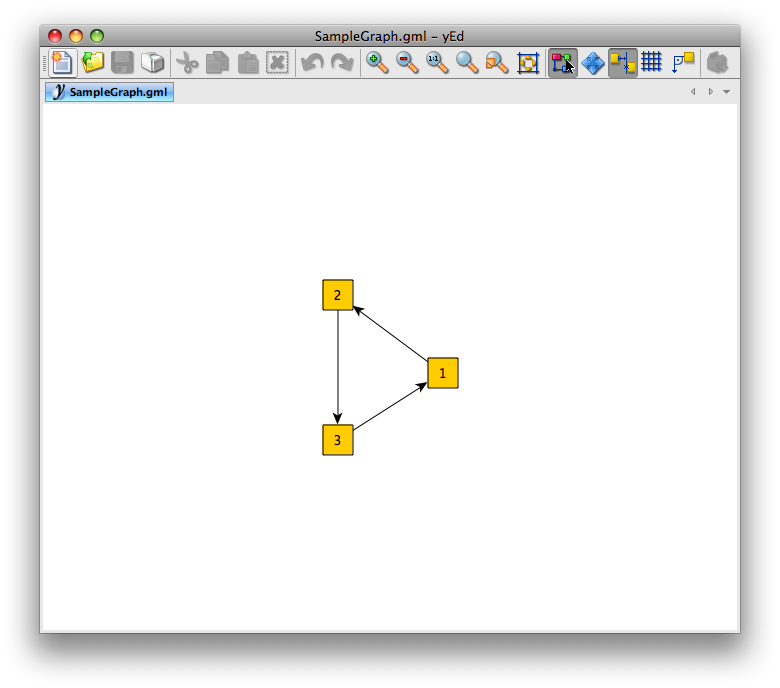
\includegraphics[scale=0.5]{pictures/SampleGraph.png}
\caption{Manual visualization of the sample graph}
\label{fig:sample_graph_yed_vis}
\end{figure}

Listing of the more complex graph with additional properties and is in the Appendix~A and the visualization of this graph shown in Figure~\ref{fig:yed_graph_vis}

\begin{figure}[h!]
\centering
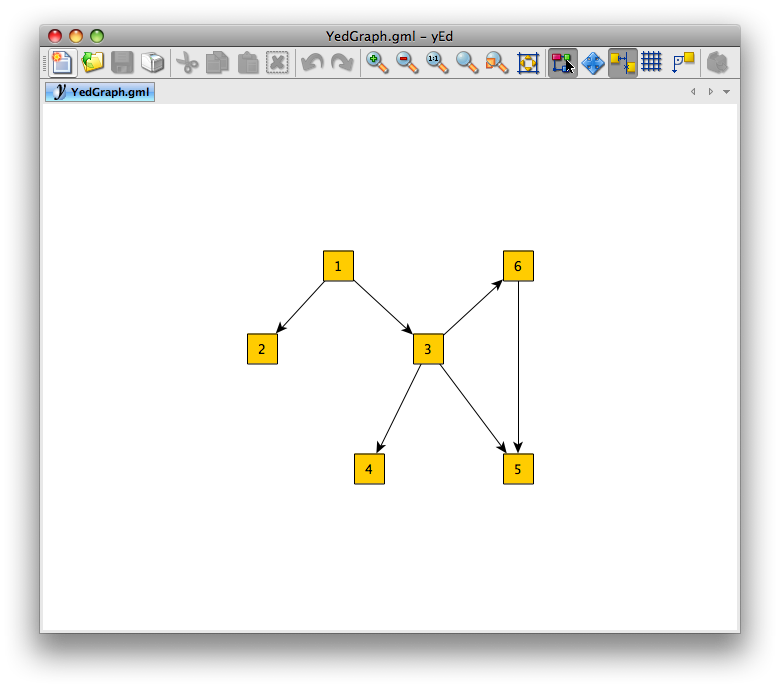
\includegraphics[scale=0.5]{pictures/YedGraph.png}
\caption{Manual visualization of the sample graph}
\label{fig:yed_graph_vis}
\end{figure}

Applications supporting GML~\cite{GML_wiki}

\begin{itemize}
\item Clairlib~\cite{clairlib}, a suite of open-source Perl modules intended to simplify a number of generic tasks in natural language processing (NLP), information retrieval (IR), and network analysis (NA).
\item Cytoscape~\cite{Cytoscape}, an open source bioinformatics software platform for visualizing molecular interaction networks, loads and save previously-constructed interaction networks in GML.
\item NetworkX~\cite{NetworkX}, an open source Python library for studying complex graphs.
\item ocamlgraph\cite{ocamlgraph}, a graph library for OCaml.
\item OGDF\cite{OGDF}, the Open Graph Drawing Framework, an open source C++ library containing implementations of various graph drawing algorithms. The library is self contained; optionally, additional packages like LP-solvers are required for some implementations.
\item Tulip~\cite{Tulip} (software) is a free software in the domain of information visualization capable of manipulating huge graphs (with more than 1.000.000 elements).
\item yEd~\cite{yed}, a free Java-based graph editor, supports import from and export to GML.
\end{itemize}

\subsection{Other Graph File Formats}

We choose to use GML because it is powerful enough for our needs and easy to implement. The next section covers several different graph file format we tried during the research. They are explained in descending order of interest.

\subsubsection{GraphML}
GraphML is a comprehensive and easy-to-use file format for graphs. It consists of a language core to describe the structural properties of a graph and a flexible extension mechanism to add application-specific data.~\cite{GraphML} Its main features include support of:
\begin{itemize}
\item directed, undirected, and mixed graphs;
\item hyper graphs;
\item hierarchical graphs;
\item graphical representations;
\item references to external data;
\item application-specific attribute data;
\item light-weight parsers;
\end{itemize}

The GraphML document consists of a graphml element and a variety of sub elements: graph, node, edge. Figure~\ref{fig:simple_graphml} below is a simple graph. It contains 11 nodes and 12 undirected edges.

\begin{figure}[h!]
\centering
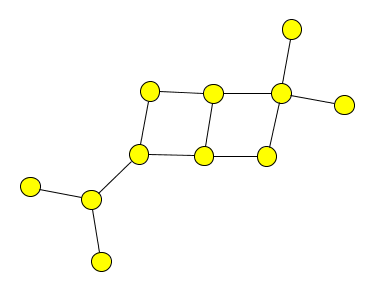
\includegraphics[scale=1.0]{pictures/simple.png}
\caption{A simple graph}
\label{fig:simple_graphml}
\end{figure}


And a corresponded graphml file is shown in Listing~\ref{simple_graphml_file}

\begin{center}
\renewcommand{\thelstlisting}{\thesection.\arabic{lstlisting}}
\begin{lstlisting} [language=xml, tabsize=1, caption={Simple graphml file}, captionpos=b, label=simple_graphml_file]
<graphml>
  <graph id="SampleGraph" edgedefault="undirected">
    <node id="node0"/>
    <node id="node1"/>
    <node id="node2"/>
    <node id="node3"/>
    <node id="node4"/>
    <node id="node5"/>
    <node id="node6"/>
    <node id="node7"/>
    <node id="node8"/>
    <node id="node9"/>
    <node id="node10"/>
    <edge source="node0" target="node2"/>
    <edge source="node1" target="node2"/>
    <edge source="node2" target="node3"/>
    <edge source="node3" target="node5"/>
    <edge source="node3" target="node4"/>
    <edge source="node4" target="node6"/>
    <edge source="node6" target="node5"/>
    <edge source="node5" target="node7"/>
    <edge source="node6" target="node8"/>
    <edge source="node8" target="node7"/>
    <edge source="node8" target="node9"/>
    <edge source="node8" target="node10"/>
  </graph>
</graphml>
\end{lstlisting}
\end{center}

GraphML support is implemented in the tool -- there is corresponded parsers to load graph from the GraphML file.

\subsubsection{DOT Graph File Format}
DOT is a plain text graph description language. It is a simple way of describing graphs in human readable form.

\begin{quotation}
``DOT graphs are typically files that end with the .gv (or .dot) extension.
At its simplest, DOT can be used to describe an undirected graph.
An undirected graph shows simple relations between objects, such as friendship between people.
The graph keyword is used to begin a new graph, and nodes are described within curly braces.
A double-hyphen (-\ -) is used to show relations between the nodes.''~\cite{DOT}
\end{quotation}

\begin{center}
\renewcommand{\thelstlisting}{\thesection.\arabic{lstlisting}}
\begin{lstlisting} [language=C, tabsize=1, caption={DOT file format: undirected graph}, captionpos=b]
graph graphname {
     a - - b - - c;
     b - - d;
}
\end{lstlisting}
\end{center}

Similar to undirected graphs, DOT can describe directed graphs, such as flowcharts and dependency trees.
The syntax is the same as for undirected graphs, except the digraph keyword is used to begin the graph, and an arrow ($->$) is used to show relationships between nodes.~\cite{DOT}

\begin{center}
\renewcommand{\thelstlisting}{\thesection.\arabic{lstlisting}}
\begin{lstlisting} [language=C, tabsize=1, caption={DOT file format: directed graph}, captionpos=b]
graph graphname {
     a -> b -> c;
     b -> d;
}
\end{lstlisting}
\end{center}

Visual representation of both graphs shown Figure~\ref{fig:dot_graphs} below.

\begin{figure}[h!]
\centering
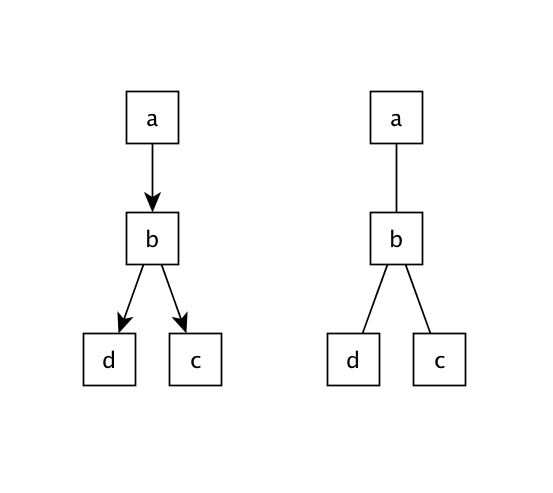
\includegraphics[scale=0.3]{pictures/dot_graph.png}
\caption{Directed and undirected graphs}
\label{fig:dot_graphs}
\end{figure}

\subsubsection{DGML}
DGML is an XML-based file format for directed graphs. Here is what a simple directed graph with three nodes and two links between them looks like

\begin{center}
\renewcommand{\thelstlisting}{\thesection.\arabic{lstlisting}}
\begin{lstlisting} [language=xml, tabsize=1, caption={DGML file format}, captionpos=b]
<?xml version="1.0" encoding="utf-8"?>
<directedGraph>
  <nodes>
    <node id="1" label="a" size="10"/>
    <node id="2" label="b" background="#FF008080"/>
    <node id="3" label="c" start="2010-06-10"/>
  </nodes>
  <links>
    <link source="1" target="2"/>
    <link source="2" target="3"/>
  </links>
  <properties>
    <property id="background" datatype="Brush"/>
    <property id="label" datatype="String"/>
    <property id="size" datatype="String"/>
    <property id="start" datatype="DateTime"/>
  </properties>
</directedGraph>
\end{lstlisting}
\end{center}

The complete XSD schema for DGML is available at Microsoft Schema web page~\cite{DGML_XSD_URL}.
DGML not only allows describing nodes and links in a graph,
but also annotating those nodes and links with any user defined property and/or category.

\subsubsection{GXL}
GXL (Graph eXchange Language) is an XML based exchange format for several kinds of graph information.
GXL provides a standardized notation for exchanging instance data (graph) including their structure (graph schema).

\begin{quotation}
``GXL was created to fulfill the need to exchange data between re-engineering tools.
Previously, interoperability between tools relied on converters between local formats.
This approach requires case-by-case negotiation of exchange semantics.
As the research area matured, it became apparent that a standard exchange format
was needed and that this format should provide a mechanism to help articulate semantics.''~\cite{GXL}.
\end{quotation}

GXL is considered as possible solution to transport graph data from different graph file formats

\subsubsection{SVG}
SVG is open graphical data storage format. Has been in development since 1999 by a group of companies within the W3C. SVG drew on experience from the designs of two older formats: Precision Graphics Markup Language (PGML) developed from Adobe's PostScript and Vector Markup Language (VML) developed from Microsoft's RTF. Which were submitted to W3C in 1998.


SVG allows three types of graphic objects:
\begin{itemize}
\item Vector graphics
\item Raster graphics
\item Text
\end{itemize}

\begin{quotation}
``Graphical objects, including PNG and JPEG raster images, can be grouped, styled, transformed,
and composited into previously rendered objects. SVG does not directly support z-indices
that separate drawing order from document order for overlapping objects, unlike some other vector mark up languages like VML.
Text can be in any XML name space suitable to the application, which enhances search ability and accessibility of the SVG graphics.
The feature set includes nested transformations, clipping paths, alpha masks, filter effects, template objects and extensibility..''~\cite{SVG}
\end{quotation}

As described above current information storage format is not meant to store graphs but is considered as possible data exchange storage format for the export functionality -- export graph visualization in the file to view it in any modern browser.

\subsection{OpenGL Visualization Standard}
\label{sec:opengl}
During first attempts to visualize data using available libraries the performance became a bottleneck. Without any measurement methods it was obvious that Java3D API used in the most of the libraries does not allow smooth intersections and real-time computations.


As possible solutions we introduces our own abstraction for visualization using OpenGL and underlying hardware acceleration.


OpenGL is a software interface to graphics hardware. This interface consists of about 120 distinct commands,
which you use to specify the objects and operations needed to produce interactive three-dimensional applications.
OpenGL is designed to work efficiently even if the computer that displays the graphics you create is not the computer that runs your graphics program.

\begin{quotation}
``OpenGL is designed as a streamlined, hardware-independent interface to be implemented on many different hardware platforms.
To achieve these qualities, no commands for performing windowing tasks or obtaining user input are included in OpenGL;
instead, you must work through whatever windowing system controls the particular hardware you're using.
Similarly, OpenGL doesn't provide high-level commands for describing models of three-dimensional objects.
Such commands might allow you to specify relatively complicated shapes such as automobiles, parts of the body, airplanes,
or molecules. With OpenGL, you must build up your desired model from a small set of geometric primitive --- points,
lines, and polygons.''~\cite{THE_RED_BOOK}
\end{quotation}

Since OpenGL is not bound to actual hardware but it is implemented as native C library and coupled to the Operation System it is run on. To avoid direct calls from the Java program to native API (Java Native Interface) we used wrapper.

There are many wrappers over OpenGL for developing on different programming languages.
One of the favorite in the Java community are JOGL and LWJGL.

\begin{quotation}
``The Lightweight Java Game Library (LWJGL) is a solution aimed directly at professional and amateur Java programmers
alike to enable commercial quality games to be written in Java. LWJGL provides developers access to
high performance cross platform libraries such as OpenGL and OpenAL (Open Audio Library) allowing for state of the art
3D games and 3D sound. Additionally LWJGL provides access to controllers such as Gamepads, Steering wheel and Joysticks.
All in a simple and straight forward API.
LWJGL is available under a BSD license, which means it is open source and freely available at no charge.''~\cite{LWJGL}
\end{quotation}


In the thesis used JOGL wrapper library over OpenGL. Java OpenGL (JOGL) is a wrapper library that allows OpenGL to be used in more Java way. Here is the overview of the JOGL project:

\begin{quotation}
``The base OpenGL C API and associated operation system API, are accessed in JOGL via Java Native Interface (JNI) calls.
As such, the underlying system must support OpenGL for JOGL to work.
JOGL differs from some other Java OpenGL wrapper libraries in that it merely exposes the procedural OpenGL API
via methods on a few classes, rather than trying to map OpenGL functionality onto the object-oriented programming paradigm.
Indeed, most of the JOGL code is auto generated from the OpenGL C header files via a conversion tool named GlueGen,
which was programmed specifically to facilitate the creation of JOGL.

This design decision has both its advantages and disadvantages.
The procedural and state machine nature of OpenGL is inconsistent with the typical method of programming under Java,
which is bothersome to many programmers. However, the straightforward mapping of the OpenGL C API to Java methods
makes conversion of existing C applications and example code much simpler.
The thin layer of abstraction provided by JOGL makes runtime execution quite efficient,
but accordingly is more difficult to code compared to higher-level abstraction libraries like Java3D.
Because most of the code is auto generated.''~\cite{JOGL}
\end{quotation}


\subsection{Program Architecture}

An overview on the tool's architecture is given in Figure~\ref{fig:modules}. The implementation is divided into several modules specialized for various tasks.
The \textsf{IO} module implements data loading from gml files. The data is stored in extended gml file format,
which contains additional properties for nodes, such as the node label.
The \textsf{Graph Core} module extends the JUNG graph model~\cite{JUNG} in order to fit it to our requirements.
The implementation of Swing GUI and OpenGL user interactions is realized by the \textsf{User Interaction} module.
The \textsf{Graph Visualization} module and its submodules contain all code for the whole visualization process,
including our own layout implementation, primitive drawing abstraction, and program state machine.
One of the most important modules of \tool\ is of course \textsf{Subgraph Extraction} that contains the implementation of the subtree calculation algorithm.

\begin{figure}[h!]
\centering
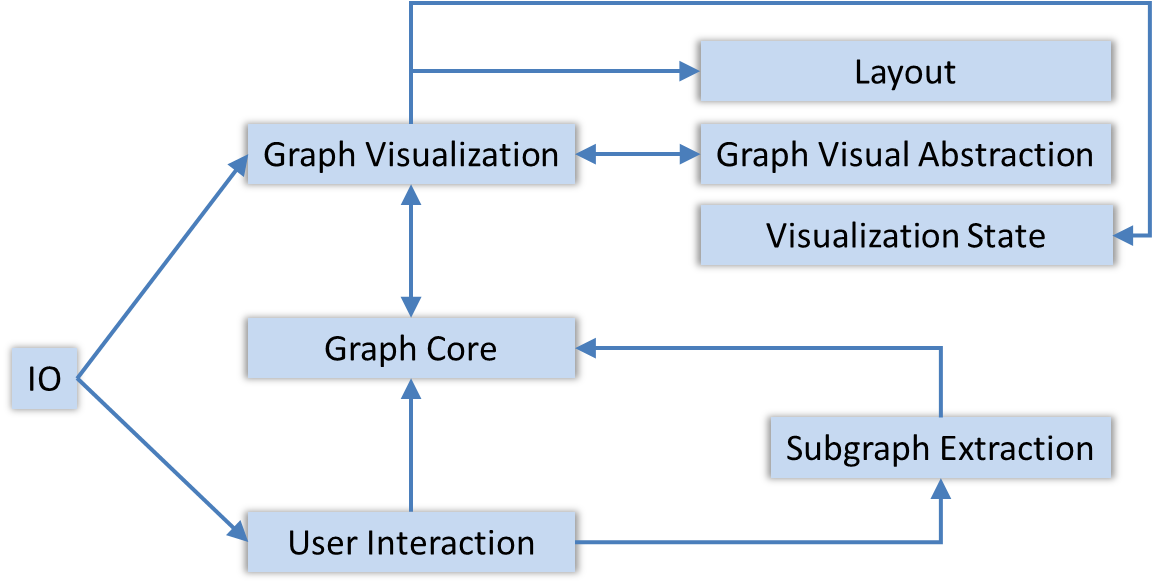
\includegraphics[scale=0.6]{pictures/modules.png}
\caption{Module architecture of GoClusterViz tool}
\label{fig:modules}
\end{figure}

One of the main module in the program is \textsf{Subgraph Extraction} module. Extraction algorithm was explained in Section~\ref{sec:algorithm} and in the Appendix~A is pseudo-code, implementation is in the class \textsf{se.lnu.thesis.algorithm.Extractor}.

Complete UML class diagram of the GoClusterViz can be found in the Appendix~C. Here is a brief overview of the package content.

Main class and program entry point is class --- \textsf{GoClusterViz}.

Package \textsf{se.lnu.thesis.gui} contains all interface abstractions and Swing implementations for main window, menus and event handling.

\textsf{se.lnu.thesis.element} is hierarchy for graph visualization. It is implementation of the Composite pattern:

\begin{quotation}
``In software engineering, the composite pattern is a partitioning design pattern.
The composite pattern describes that a group of objects are to be treated in the same way as a single instance of an object.
The intent of a composite is to `compose' objects into tree structures to represent part-whole hierarchies.
Implementing the composite pattern lets clients treat individual objects and compositions uniformly.''~\cite{COMPOSITE_GAMMA}
\end{quotation}

\begin{figure}[h!]
\centering
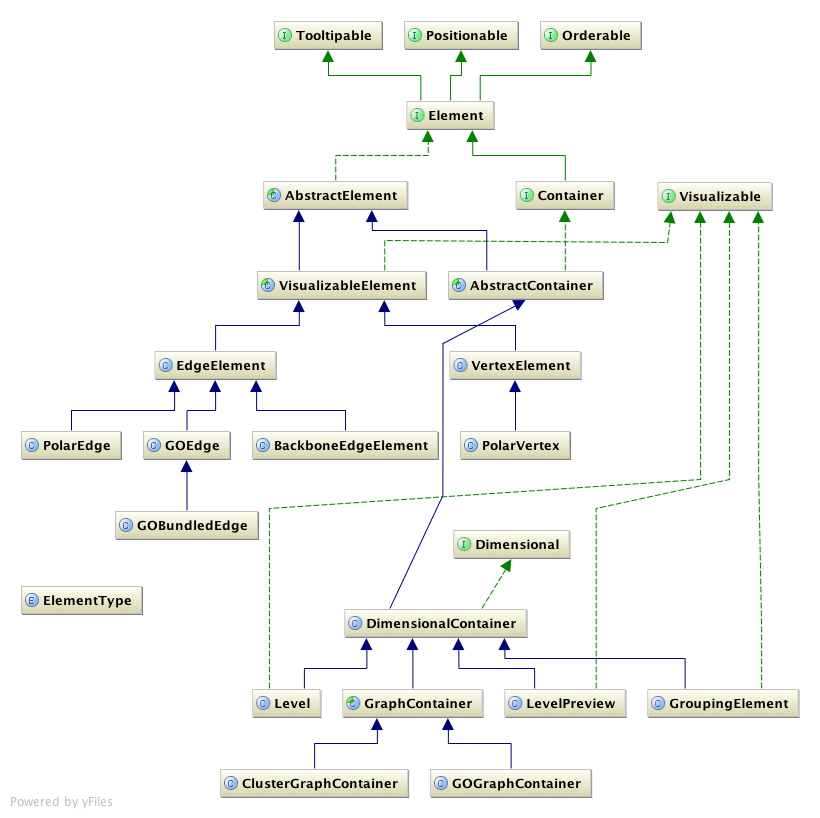
\includegraphics[scale=0.4]{pictures/uml_elements.png}
\caption{Graph elements visualisation hierarchy abstraction}
\label{fig:uml_elements}
\end{figure}

Package \textsf{se.lnu.thesis.paint} contains all drawing implementations.
Graph elements do not implement visualization shape, for that purpose there is \textsf{ElementVisualizer} abstraction. Diagram in Figure~\ref{fig:uml_visualizers} shows complete UML diagram of the package \textsf{se.lnu.thesis.paint.visualizer}, there are several different shape visualizer. To reduce memory usage all visualizers are stored in the \textsf{ElementVisualizerFactory} --- Flyweight design pattern.

\begin{quotation}
``Flyweight is a software design pattern.
A flyweight is an object that minimizes memory use by sharing as much data as possible with other similar objects;
it is a way to use objects in large numbers when a simple repeated representation would use an unacceptable amount of memory.
The term is named after the boxing weight class.
Often some parts of the object state can be shared and it is common to put them in external data structures and pass them to
the flyweight objects temporarily when they are used.''~\cite{FLYWEIGHT}
\end{quotation}

Flyweight pattern is used to store different kind of visualizers for graph elements. It means for each element of the graph there is a reference to visualizer object containing its shape, metrics, and other formatting data, which reduce amount of data to hundreds or thousands of bytes for each character. For every element of the graph there is a reference to a flyweight visualizer object shared by every instance of the same graph element in the graph; only the position of each element and current state (selected, highlighted, focused) is stored internally.

\begin{figure}[h!]
\centering
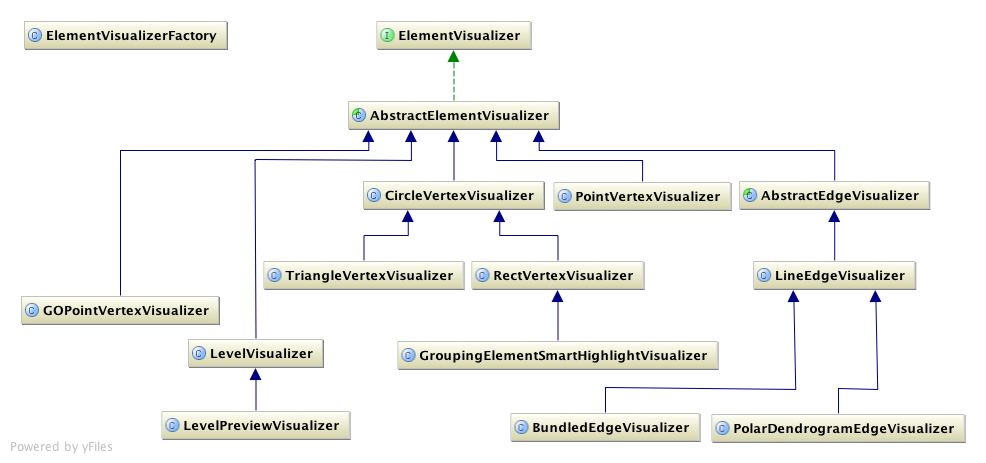
\includegraphics[scale=0.35]{pictures/uml_visualizers.png}
\caption{Flyweight element visualizers}
\label{fig:uml_visualizers}
\end{figure}

User interaction state machine is implementation of the State software development pattern located in the package \textsf{se.lnu.thesis.paint.state}.

\begin{quotation}
``A monolithic objects behavior is a function of its state, and it must change its behavior at run-time depending on that state.
Or, an application is characterized by large and numerous case statements that vector flow of control based on the state
of the application. The State pattern does not specify where the state transitions will be defined. The choices are two:
the context object, or each individual State derived class.
The advantage of the latter option is ease of adding new State derived classes.
The disadvantage is each State derived class has knowledge of (coupling to) its siblings,
which introduces dependencies between subclasses.
A table-driven approach to designing finite state machines does a good job of specifying state transitions,
but it is difficult to add actions to accompany the state transitions. The pattern-based approach uses code
(instead of data structures) to specify state transitions,
but it does a good job of accommodating state transition actions.''~\cite{STATE}
\end{quotation}

It means that graph has several states: normal view, zoomed view, lens is on the scene, etc.
It releases the code from the long ``switch'' statements  and determines logic into different classes.

\begin{figure}[h!]
\centering
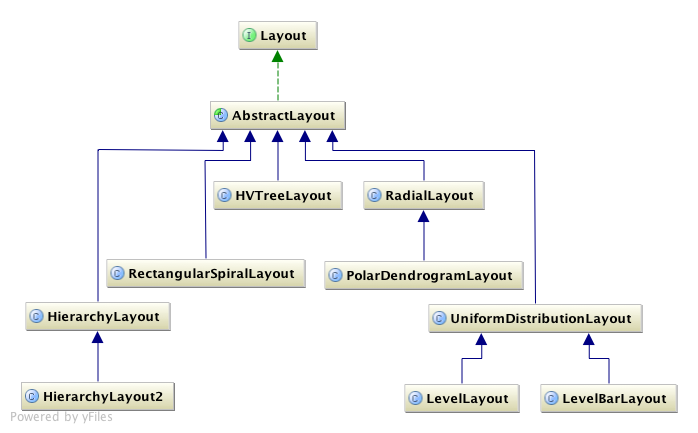
\includegraphics[scale=0.5]{pictures/uml_layouts.png}
\caption{Layouts class diagram}
\label{fig:uml_layouts}
\end{figure}


During this work several layouts were implemented, as it was discussed earlier.
Layout implementations are in the \textsf{se.lnu.thesis.layout} package. UML class diagram is shown on Figure~\ref{fig:uml_layouts}.